\documentclass[a4paper, 11pt, oneside]{article}

\newcommand{\plogo}{\fbox{$\mathcal{PL}$}} 
\usepackage{amsmath}
\usepackage[utf8]{inputenc} 
\usepackage[T1]{fontenc} 
\usepackage{enumitem}
\usepackage{graphicx}
\usepackage{graphicx}
\usepackage{supertabular}
\usepackage{biblatex}
\usepackage{hyperref}
\usepackage{dirtytalk}
\usepackage[spanish]{babel}
\graphicspath{{Imagenes/}}

\begin{document} 

\begin{titlepage} 

	\centering 
	
	\scshape 
	
	\vspace*{\baselineskip} 
	
	
	
	\rule{\textwidth}{1.6pt}\vspace*{-\baselineskip}\vspace*{2pt} 
	\rule{\textwidth}{0.4pt} 
	
	\vspace{0.75\baselineskip} 
	
	{\LARGE Practica 8: Security-Enhanced Linux (SElinux)}	
	\vspace{0.75\baselineskip} 
	
	\rule{\textwidth}{0.4pt}\vspace*{-\baselineskip}\vspace{3.2pt}
	\rule{\textwidth}{1.6pt} 
	
	\vspace{2\baselineskip} 
	

	ADMINISTRACIÓN DE SISTEMAS UNIX/LINUX
	
	\vspace*{1\baselineskip} 
	
	
	
	Alumna:
	
	\vspace{0.2\baselineskip} 
	
	{\scshape\Large Karla Adriana Esquivel Guzmán url{https://github.com/karlycaramelo} \\
    Eric Giovanni Miguel Torres url{https://github.com/EricGiovanni}\\ 
    María Ximena Lezama Hernández url{https://github.com/LezamaXi}\\ 
    Gonzalo Vazquez Cruz url{https://github.com/truerandom}}
	\vspace{0.5\baselineskip} 
	\vfill
	
\includegraphics[scale=0.65]{unam.jpg}
	
	\textit{UNIVERSIDAD NACIONAL AUTONOMA DE MEXICO} 
	
	
	
	
	
	\vspace{0.3\baselineskip} 
	
	13/Mayo/2019 
	
	 

\end{titlepage}

\begin{enumerate}
    \item[1.] Al instalar CentOS, por default crea los siguientes usuarios: sysadm\_u, system\_u,
    xguest\_u, root, guest\_u, staff\_u, user\_u y unconfined\_u. Investiga cuales son las
    diferencias entre ellos y con que comandos puedo ver que tiene permitido cada uno de
    ellos.
    \begin{itemize}
        \item \textbf{sysadm\_u:} Usuario SELinux con rol administrativo directo en el sistema asignado. Es utilizado para cuentas de Linux que solo realizan tareas administrativas.
        
        \item \textbf{system\_u:} Usuario especial de SELinux destinado a servicios de sistemas. No es utilizado directamente.
        
        \item \textbf{xguest\_u:} Se define en la política como un usuario sin privilegios. SELinux evita que los usuarios sin privilegios realicen tareas de administración sin pasar a una función diferente.

        \item \textbf{root:} El usuario de SELinux destinado para la cuenta de root. Éste es utilizado para la cuenta de root de Linux.
        
        \item \textbf{guest\_u:} La descripción de este usuario es la misma que $xguest\_u$.
        
        \item \textbf{staff\_u:} Usuario SELinux para operadores que necesitan ejecutar tanto comandos no administrativos (a través del rol staff\_r) como comandos administrativos (a través del rol sysadm\_r). Se utiliza para cuentas de Linux utilizadas tanto para el uso del usuario final como para tareas administrativas.
        
        \item \textbf{user\_u:} Usuario SELinux para cuentas no privilegiadas.
        
        \item \textbf{unconfined\_u:} Usuario de SELinux destinado a usuarios no restringidos. Los usuarios no confinados casi no tienen restricciones en el contexto de SELinux y están destinados a sistemas en los que solo los servicios con acceso a Internet deben ejecutarse confinados (es decir, el almacén de políticas de SELinux dirigido). Se usa para todos los usuarios en un sistema de destino.

    \end{itemize}
    \item[2.] Al crear un usuario de linux en un sistema con SELinux por default se le asigna un
    usuario de SELinux. ¿En qué tipo de sistemas convendría los usuarios que tiene por
    default CentOS? Cambia el usuario por default de SELinux que se asigna en CentOS.\\ \textbf{Respuesta:}
    \begin{itemize}
        \item De acuerdo a lo que sabemos hasta ahora convendría en un sistema en el cual los usuarios necesitan ejecutar las tareas confinadamente.\\ \say{Casi todos los servicios que escuchan en una red, como sshd o httpd, están confinados en una red. Además, la mayoría de los procesos que se ejecutan como usuario root y realizan tareas para los usuarios, como la utilidad passwd, están limitados. Cuando un proceso está limitado, se ejecuta en su propio dominio, como el proceso httpd que se ejecuta en el dominio httpd\_t. Si un atacante compromete un proceso confinado, según la configuración de la política de SELinux, el acceso de un atacante a los recursos y el posible daño que pueden hacer es limitado.}
    
        \item El usuario por default de SELinux es \textbf{unconfined\_u} lo cambiamos a \textbf{system\_u}
            \begin{center}
                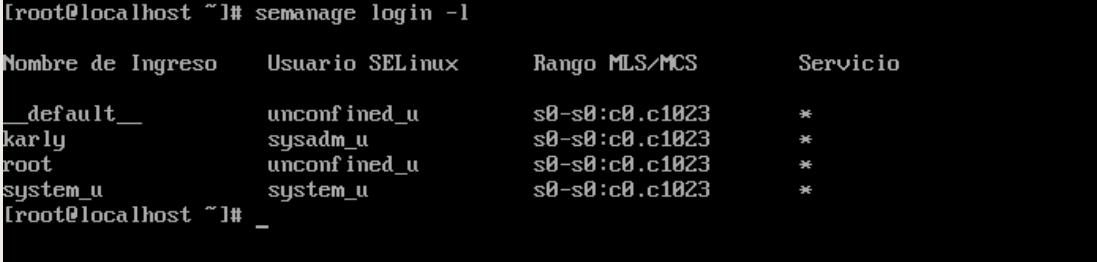
\includegraphics[scale=0.25]{CentOS2.png}
            \end{center}
        Para cambiar el usuario de SELinux por default, utilizamos el siguiente comando
    \begin{verbatim}
        semanage login -a -s system_u __default__
    \end{verbatim}
    Nuevamente escribimos en la terminal \textbf{semanage login -l} para que nos muestre la lista de usuarios de SELinux y ya aparece el cambio para el usuario por default.
    \begin{center}
        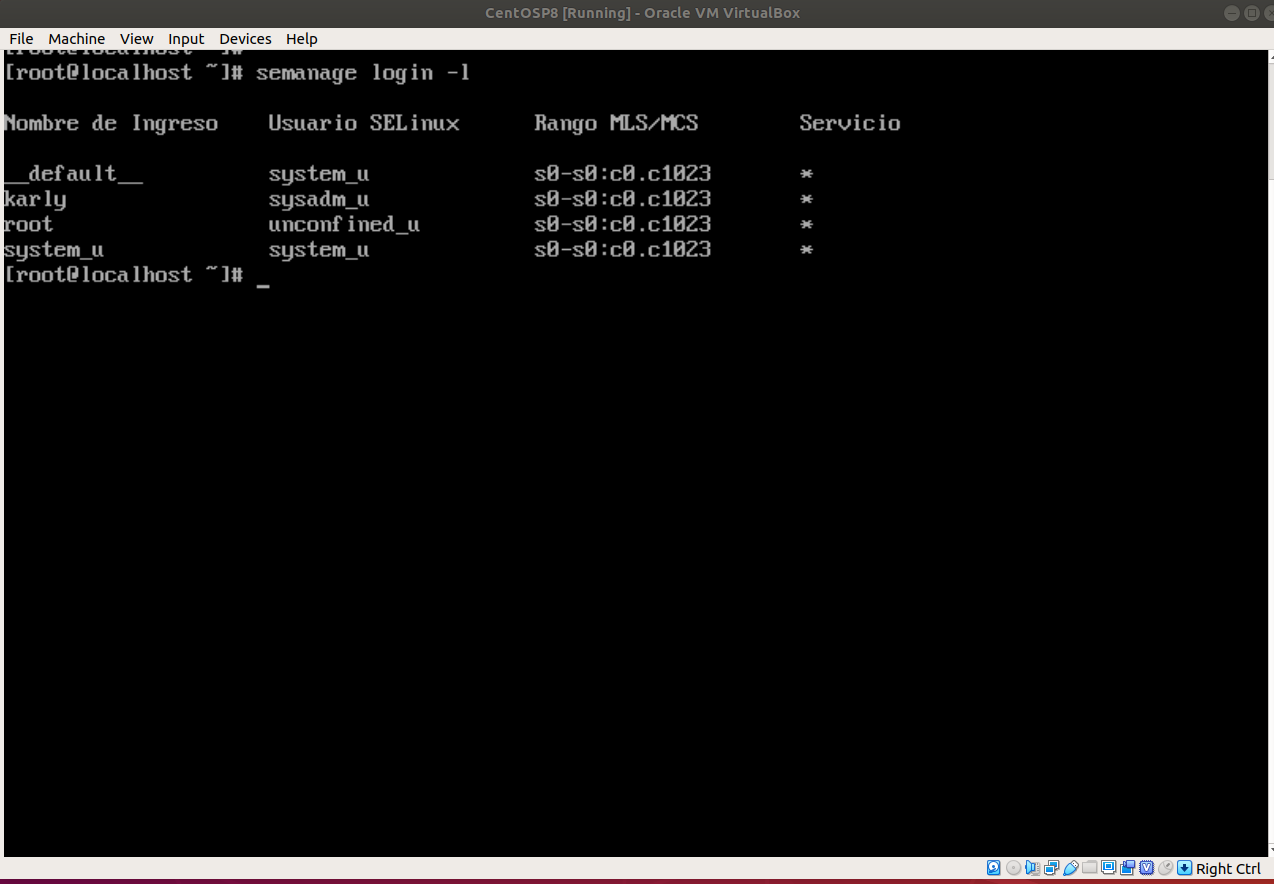
\includegraphics[scale=0.22]{CentOS3.png}
    \end{center} 
    \end{itemize}
    
    \item[3.] Investiga el comando auditallow, ¿para qué sirve? ¿Cómo se usa? Da un ejemplo de
    uso.
    \begin{itemize}
        \item \textbf{auditallow}, nos permite controlar la auditoría de los intentos de acceso permitidos. A diferencia del acceso denegado, el acceso permitido no se registra de forma predeterminada. La regla auditallow no permite el acceso; Sólo permite la auditoría de los permisos permitidos. (Registro de los accesos).

        \item Se utiliza de la siguiente forma:
    \begin{verbatim}
    auditallow user_t bin_t : file execute;    
    \end{verbatim}
        En este ejemplo auditalow tiene el tipo de origen user\_t, el tipo de destino bin\_t, el archivo de clase de objeto y la ejecución de permisos. Esta regla se puede leer como "Permite auditar al user\_t los archivos de tipo bin\_t".

        
    \end{itemize}
    \item[4.] Crea un usuario tal que solamente pueda tener acceso a su carpeta home. Si el nombre
    de usuario es user entonces se debe agregar un tipo de archivo user\_t y todos los
    archivos de dicho usuario deben tener ese tipo.\\
    Se crea el usuario para linux con el comando useradd,  en este caso para crearlo en SELinux basta simplemente con mapear al usuario llamado user al tipo de usuario user\_u  puesto que este tipo cumple con las especificaciones que se piden en este inciso. El comando que se utiliza para el mapeo es el siguiente:
    \begin{verbatim}
        semanage login -a -s user_u user
    \end{verbatim}
    \begin{center}
        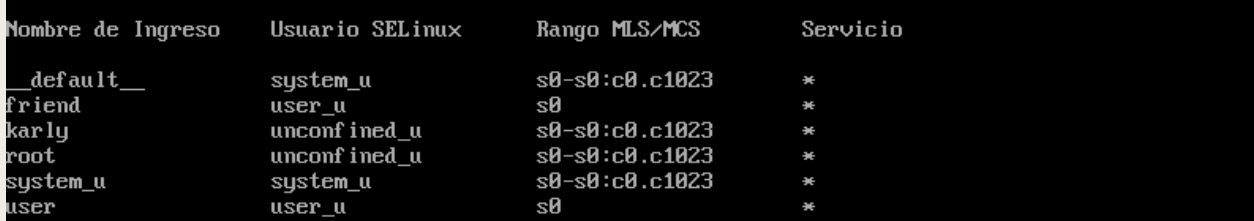
\includegraphics[scale=0.25]{CentOS4.png}
        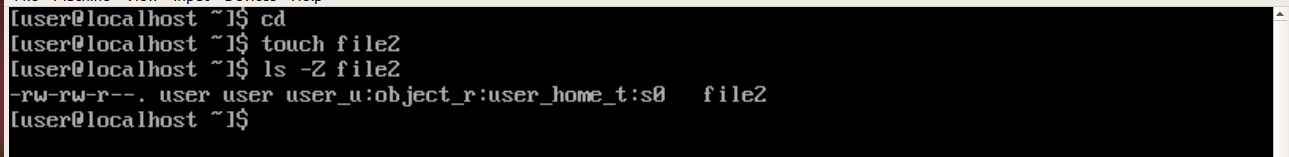
\includegraphics[scale=0.25]{CentOS5.png}
    \end{center}
    
    \item[5.] Dependiendo de los requerimientos del sistema, a ciertos usuarios, procesos o carpetas
    pueden tener acceso o no a recursos del sistema. Crea dos reglas de SELinux.
\end{enumerate}

\begin{thebibliography}{X}
\bibitem{Lib} SELinux by Example: Using Security Enhanced Linux, Frank Mayer, Karl MacMillan,, David Caplan, Julio 27, 2006.
\bibitem{sys} \url{https://www.systutorials.com/docs/linux/man/8-guest_selinux/}.
\bibitem{wiki} \url{https://wiki.gentoo.org/wiki/SELinux/Users_and_logins}
\bibitem{red} \url{https://access.redhat.com/documentation/en-us/red_hat_enterprise_linux/6/html/security-enhanced_linux/index}
\bibitem{chcon} \url{https://www.thegeekstuff.com/2017/07/chcon-command-examples/}
\end{thebibliography}
\end{document}